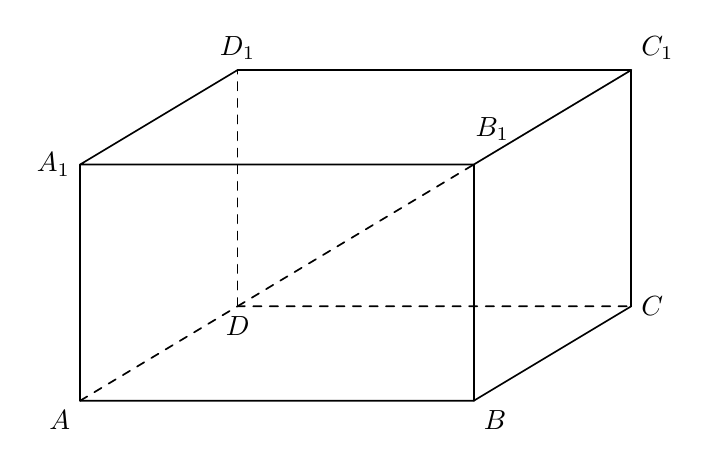
\begin{tikzpicture}[line width=0.6pt, line join=round, line cap=round]
  \coordinate (A) at (0,0);
  \coordinate (B) at (5,0);
  \coordinate (D) at (2,1.2);
  \coordinate (C) at (7,1.2);
  \coordinate (A1) at (0,3);
  \coordinate (B1) at (5,3);
  \coordinate (D1) at (2,4.2);
  \coordinate (C1) at (7,4.2);
  % bottom / top
  \draw (A) -- (B) -- (C);
  \draw[dashed] (A) -- (D) -- (C);
  \draw (A1) -- (B1) -- (C1) -- (D1) -- cycle;
  % verticals
  \draw (A) -- (A1);
  \draw (B) -- (B1);
  \draw (C) -- (C1);
  \draw[dashed] (D) -- (D1);
  % body diagonal
  \draw[dashed] (D) -- (B1);
  % labels
  \node[below left] at (A) {$A$};
  \node[below right] at (B) {$B$};
  \node[below] at (D) {$D$};
  \node[right] at (C) {$C$};
  \node[left] at (A1) {$A_{1}$};
  \node[above right,xshift=-3pt,yshift=5pt] at (B1) {$B_{1}$};
  \node[above] at (D1) {$D_{1}$};
  \node[above right] at (C1) {$C_{1}$};
\end{tikzpicture}
